\documentclass{standalone}
\usepackage{tikz}
\usetikzlibrary{patterns, positioning}
\usepackage[sfdefault]{ClearSans} %% option 'sfdefault' activates Clear Sans as the default text font
\usepackage[T1]{fontenc}

\begin{document}
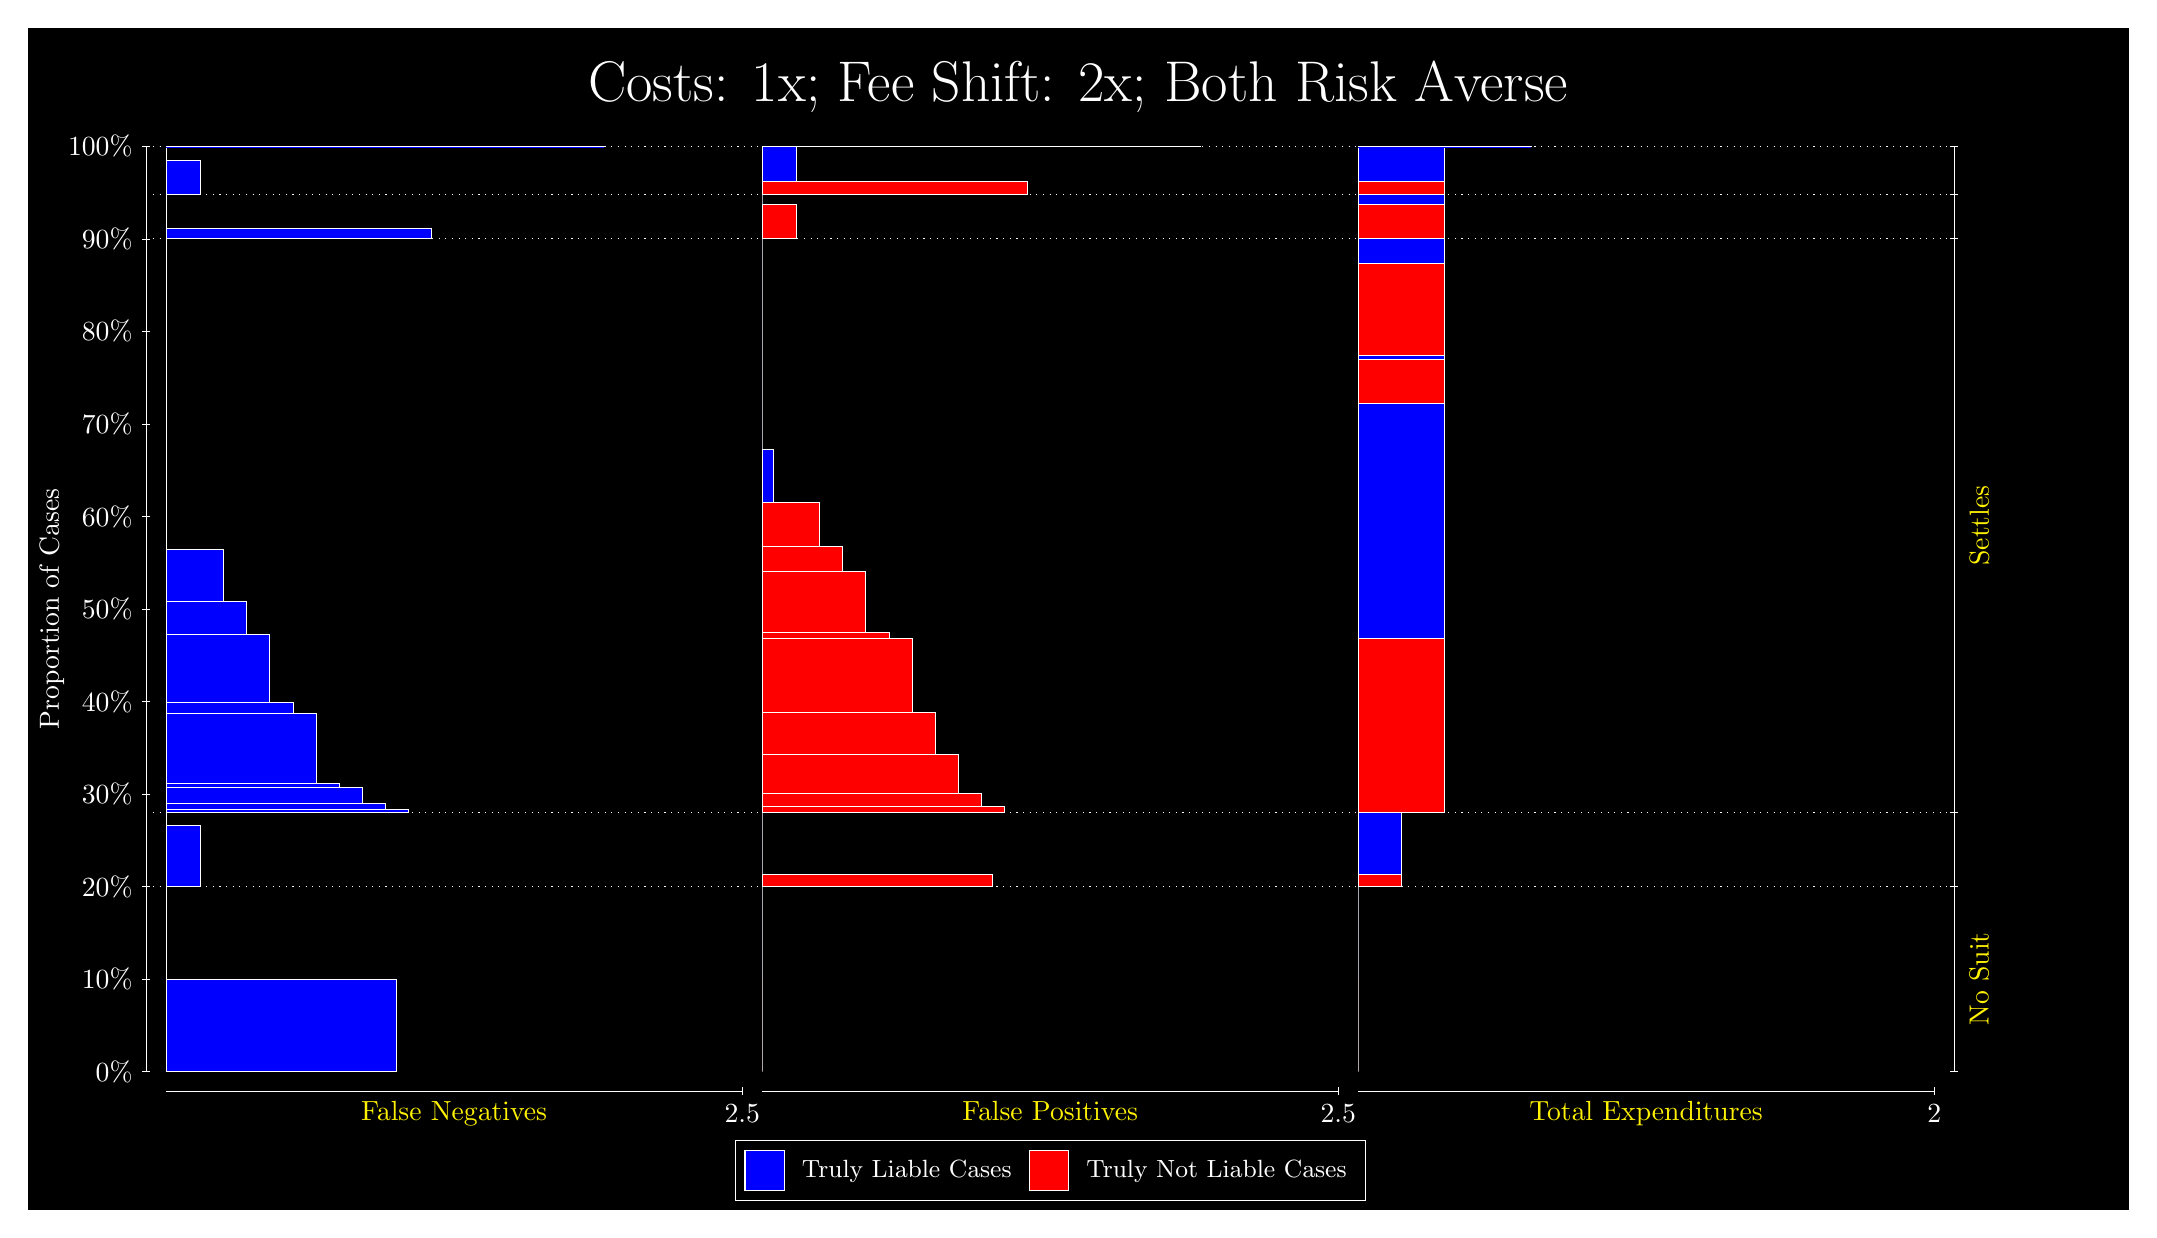
\begin{tikzpicture}
\draw[fill=black] (0,0) rectangle (26.667,15);
\draw[text=white] (0,13.5) rectangle (26.667,15) node[midway] {\huge Costs: 1x; Fee Shift: 2x; Both Risk Averse};
\draw[white, very thin] (1.5,1.75) -- (1.5,13.5);
\node[rotate=90, text=white, anchor=center] at (0.3, 7.625) {Proportion of Cases};
\draw[white, very thin] (1.45,1.75) -- (1.55,1.75);
\node[text=white, anchor=east] at (1.45, 1.75) {0\%};
\draw[white, very thin] (1.45,2.925) -- (1.55,2.925);
\node[text=white, anchor=east] at (1.45, 2.925) {10\%};
\draw[white, very thin] (1.45,4.1) -- (1.55,4.1);
\node[text=white, anchor=east] at (1.45, 4.1) {20\%};
\draw[white, very thin] (1.45,5.275) -- (1.55,5.275);
\node[text=white, anchor=east] at (1.45, 5.275) {30\%};
\draw[white, very thin] (1.45,6.45) -- (1.55,6.45);
\node[text=white, anchor=east] at (1.45, 6.45) {40\%};
\draw[white, very thin] (1.45,7.625) -- (1.55,7.625);
\node[text=white, anchor=east] at (1.45, 7.625) {50\%};
\draw[white, very thin] (1.45,8.8) -- (1.55,8.8);
\node[text=white, anchor=east] at (1.45, 8.8) {60\%};
\draw[white, very thin] (1.45,9.975) -- (1.55,9.975);
\node[text=white, anchor=east] at (1.45, 9.975) {70\%};
\draw[white, very thin] (1.45,11.15) -- (1.55,11.15);
\node[text=white, anchor=east] at (1.45, 11.15) {80\%};
\draw[white, very thin] (1.45,12.325) -- (1.55,12.325);
\node[text=white, anchor=east] at (1.45, 12.325) {90\%};
\draw[white, very thin] (1.45,13.5) -- (1.55,13.5);
\node[text=white, anchor=east] at (1.45, 13.5) {100\%};

\draw[white, very thin] (24.457,1.75) -- (24.457,13.5);
\draw[white, very thin] (24.407,1.75) -- (24.507,1.75);
\node[anchor=west] at (24.407, 1.75) {};
\draw[white, very thin] (24.407,4.1) -- (24.507,4.1);
\node[anchor=west] at (24.407, 4.1) {};
\draw[white, very thin] (24.407,5.0364) -- (24.507,5.0364);
\node[anchor=west] at (24.407, 5.0364) {};
\draw[white, very thin] (24.407,12.335) -- (24.507,12.335);
\node[anchor=west] at (24.407, 12.335) {};
\draw[white, very thin] (24.407,12.888) -- (24.507,12.888);
\node[anchor=west] at (24.407, 12.888) {};
\draw[white, very thin] (24.407,13.495) -- (24.507,13.495);
\node[anchor=west] at (24.407, 13.495) {};
\draw[white, very thin] (24.407,13.497) -- (24.507,13.497);
\node[anchor=west] at (24.407, 13.497) {};
\draw[white, very thin] (24.407,13.5) -- (24.507,13.5);
\node[anchor=west] at (24.407, 13.5) {};

\draw[white, very thin, fill=blue] (1.75,1.75) rectangle (4.6775,2.925);
\draw[white, very thin, fill=red] (1.75,2.925) rectangle (1.75,4.1);
\draw[white, very thin, fill=blue] (1.75,4.1) rectangle (2.1891,4.8752);
\draw[white, very thin, fill=red] (1.75,4.8752) rectangle (1.75,5.0364);
\draw[white, very thin, fill=blue] (1.75,5.0364) rectangle (4.8239,5.0854);
\draw[white, very thin, fill=blue] (1.75,5.0854) rectangle (4.5312,5.1554);
\draw[white, very thin, fill=blue] (1.75,5.1554) rectangle (4.2384,5.3555);
\draw[white, very thin, fill=blue] (1.75,5.3555) rectangle (3.9457,5.41);
\draw[white, very thin, fill=blue] (1.75,5.41) rectangle (3.6529,6.3025);
\draw[white, very thin, fill=blue] (1.75,6.3025) rectangle (3.3602,6.4338);
\draw[white, very thin, fill=blue] (1.75,6.4338) rectangle (3.0674,7.3049);
\draw[white, very thin, fill=blue] (1.75,7.3049) rectangle (2.7746,7.722);
\draw[white, very thin, fill=blue] (1.75,7.722) rectangle (2.4819,8.3885);
\draw[white, very thin, fill=red] (1.75,8.3885) rectangle (1.75,12.335);
\draw[white, very thin, fill=blue] (1.75,12.335) rectangle (5.1167,12.465);
\draw[white, very thin, fill=red] (1.75,12.465) rectangle (1.75,12.888);
\draw[white, very thin, fill=blue] (1.75,12.888) rectangle (2.1891,13.328);
\draw[white, very thin, fill=red] (1.75,13.328) rectangle (1.75,13.495);
\draw[white, very thin, fill=blue] (1.75,13.495) rectangle (7.3123,13.496);
\draw[white, very thin, fill=red] (1.75,13.496) rectangle (1.75,13.497);
\draw[white, very thin, fill=red] (1.75,13.497) rectangle (1.75,13.498);
\draw[white, very thin, fill=blue] (1.75,13.498) rectangle (1.75,13.5);
\draw[white, very thin, fill=red] (9.3189,1.75) rectangle (9.3189,2.925);
\draw[white, very thin, fill=blue] (9.3189,2.925) rectangle (9.3189,4.1);
\draw[white, very thin, fill=red] (9.3189,4.1) rectangle (12.246,4.2612);
\draw[white, very thin, fill=blue] (9.3189,4.2612) rectangle (9.3189,5.0364);
\draw[white, very thin, fill=red] (9.3189,5.0364) rectangle (12.393,5.1191);
\draw[white, very thin, fill=red] (9.3189,5.1191) rectangle (12.1,5.2793);
\draw[white, very thin, fill=red] (9.3189,5.2793) rectangle (11.807,5.7731);
\draw[white, very thin, fill=red] (9.3189,5.7731) rectangle (11.515,6.3121);
\draw[white, very thin, fill=red] (9.3189,6.3121) rectangle (11.222,7.2549);
\draw[white, very thin, fill=red] (9.3189,7.2549) rectangle (10.929,7.3285);
\draw[white, very thin, fill=red] (9.3189,7.3285) rectangle (10.636,8.0993);
\draw[white, very thin, fill=red] (9.3189,8.0993) rectangle (10.344,8.42);
\draw[white, very thin, fill=red] (9.3189,8.42) rectangle (10.051,8.983);
\draw[white, very thin, fill=blue] (9.3189,8.983) rectangle (9.4652,9.6494);
\draw[white, very thin, fill=blue] (9.3189,9.6494) rectangle (9.3189,12.335);
\draw[white, very thin, fill=red] (9.3189,12.335) rectangle (9.758,12.758);
\draw[white, very thin, fill=blue] (9.3189,12.758) rectangle (9.3189,12.888);
\draw[white, very thin, fill=red] (9.3189,12.888) rectangle (12.686,13.055);
\draw[white, very thin, fill=blue] (9.3189,13.055) rectangle (9.758,13.495);
\draw[white, very thin, fill=red] (9.3189,13.495) rectangle (9.3189,13.496);
\draw[white, very thin, fill=blue] (9.3189,13.496) rectangle (9.3189,13.497);
\draw[white, very thin, fill=red] (9.3189,13.497) rectangle (14.881,13.498);
\draw[white, very thin, fill=blue] (9.3189,13.498) rectangle (11.954,13.5);
\draw[white, very thin, fill=red] (16.888,1.75) rectangle (16.888,2.925);
\draw[white, very thin, fill=blue] (16.888,2.925) rectangle (16.888,4.1);
\draw[white, very thin, fill=red] (16.888,4.1) rectangle (17.437,4.2612);
\draw[white, very thin, fill=blue] (16.888,4.2612) rectangle (17.437,5.0364);
\draw[white, very thin, fill=red] (16.888,5.0364) rectangle (17.986,7.2549);
\draw[white, very thin, fill=blue] (16.888,7.2549) rectangle (17.986,10.233);
\draw[white, very thin, fill=red] (16.888,10.233) rectangle (17.986,10.796);
\draw[white, very thin, fill=blue] (16.888,10.796) rectangle (17.986,10.845);
\draw[white, very thin, fill=red] (16.888,10.845) rectangle (17.986,12.011);
\draw[white, very thin, fill=blue] (16.888,12.011) rectangle (17.986,12.335);
\draw[white, very thin, fill=red] (16.888,12.335) rectangle (17.986,12.758);
\draw[white, very thin, fill=blue] (16.888,12.758) rectangle (17.986,12.888);
\draw[white, very thin, fill=red] (16.888,12.888) rectangle (17.986,13.055);
\draw[white, very thin, fill=blue] (16.888,13.055) rectangle (17.986,13.495);
\draw[white, very thin, fill=red] (16.888,13.495) rectangle (19.083,13.496);
\draw[white, very thin, fill=blue] (16.888,13.496) rectangle (19.083,13.497);
\draw[white, very thin, fill=red] (16.888,13.497) rectangle (19.083,13.498);
\draw[white, very thin, fill=blue] (16.888,13.498) rectangle (19.083,13.5);
\draw[white, dotted] (1.5,4.1) -- (24.457,4.1);
\draw[white, dotted] (1.5,5.0364) -- (24.457,5.0364);
\draw[white, dotted] (1.5,12.335) -- (24.457,12.335);
\draw[white, dotted] (1.5,12.888) -- (24.457,12.888);
\draw[white, dotted] (1.5,13.495) -- (24.457,13.495);
\draw[white, dotted] (1.5,13.497) -- (24.457,13.497);
\draw[white, very thin] (1.75,1.5) -- (9.0689,1.5);
\node[text=yellow, anchor=north] at (5.4094, 1.5) {False Negatives};
\draw[white, very thin] (9.0689,1.45) -- (9.0689,1.55);
\node[text=white, anchor=north] at (9.0689, 1.45) {2.5};

\draw[white, very thin] (9.3189,1.5) -- (16.638,1.5);
\node[text=yellow, anchor=north] at (12.978, 1.5) {False Positives};
\draw[white, very thin] (16.638,1.45) -- (16.638,1.55);
\node[text=white, anchor=north] at (16.638, 1.45) {2.5};

\draw[white, very thin] (16.888,1.5) -- (24.207,1.5);
\node[text=yellow, anchor=north] at (20.547, 1.5) {Total Expenditures};
\draw[white, very thin] (24.207,1.45) -- (24.207,1.55);
\node[text=white, anchor=north] at (24.207, 1.45) {2};

\node[text=yellow, centered, rotate=90] at (24.777, 2.925) {No Suit};

\node[text=yellow, centered, rotate=90] at (24.777, 8.6857) {Settles};





\draw (12.978300999999998,1.5) node[draw=none] (baseCoordinate) {};
\begin{scope}[align=center]
        \matrix[scale=0.5, draw=white, below=0.5cm of baseCoordinate, nodes={draw}, column sep=0.1cm]{
            \node[rectangle, draw, minimum width=0.5cm, minimum height=0.5cm, fill=blue] {}; &
            \node[draw=none, font=\small, text=white] (B) {Truly Liable Cases}; &
            \node[rectangle, draw, minimum width=0.5cm, minimum height=0.5cm, fill=red] {}; &
            \node[draw=none, font=\small, text=white] (B) {Truly Not Liable Cases}; \\
            };
\end{scope}

\end{tikzpicture}
\end{document}